\documentclass[]{article}
\usepackage[brazil]{babel}
\usepackage{graphicx}
\usepackage{mathtools}
\usepackage{float} 
\usepackage{xcolor}


\usepackage{array}
\usepackage{booktabs}



% margenes
\usepackage[a4paper,left=3cm,right=3cm,top=3cm]{geometry}

%opening
\title{}
\author{}

\begin{document}

\begin{center}
	{\tiny {\normalsize {\large Lista de exercicios 3\\
Transferência de calor e mecânica dos fluidos computacional I\\
\textbf{Cristian Herledy Lopez Lara}}}}
\end{center}

\section*{Exercício 3.1}
\subsubsection*{4.1}

No caso das oscilações numéricas, são efeitos que surgem da utilização de sistemas de interpolação espacial linear que geram erros de truncamento (justamente por serem aproximações). No caso de oscilação, os erros associados são erros não dissipativos como os gerados pelo sistema CDS, ou os derivados da utilização de diferenças centrais. Essas oscilações aparecem aproximando valores de propriedades transportadas pelo fluxo com médias espaciais (interpolações) geram perturbações no fluxo distantes da solução real. Esses erros são atenuados com o refinamento da malha, justamente porque a aproximação é melhorada espacialmente e, portanto, o erro de truncamento associado diminui. No caso da difusão numérica, deriva do aparecimento de erros de truncamento de natureza dissipativa associados a termos advectivos. Como a interpolação não é exata, suas aproximações adicionam erros, que também podem ser tratados com o refinamento da malha, mas não eliminados.\\

\subsubsection*{4.2}

A divisão espacial, que é o próprio ato de utilizar uma malha, gera erros de truncamento ao aplicar aproximações com funções de interpolação devido à natureza discreta do uso da técnica. A verdadeira solução vem da ideia do regime contínuo. Numericamente, discretizações temporais e espaciais são usadas para chegar discretamente o mais próximo possível de uma solução completamente contínua para o problema físico. Malhas menores têm efeito direto na redução de erros de truncamento, pois a discretização se aproxima da solução contínua ou real.

\subsubsection*{4.3}

A equação unidimensional para o problema de convecção e difusão em regime permanente é

\begin{equation}
	\frac{\partial}{\partial x} \left( \rho u \phi \right) = \frac{\partial}{\partial x} \left( \Gamma^\phi \frac{\partial \phi}{\partial x} \right)
\end{equation}

Integrando no espaço obtemos\\

\begin{equation}
	 \rho u \phi _e -  \rho u \phi_w =  \varGamma^\phi \frac{\partial \phi}{\partial x}\arrowvert_e - \varGamma^\phi \frac{\partial \phi}{\partial x}\arrowvert_w
\end{equation}


Aproximando os fluxos usando diferenças centrais CDS como interpolação linear, usamos as seguintes expressões

\begin{equation}
	\begin{aligned}
		\phi_{e} = \dfrac{\phi_{E} + \phi_{P}}{2} \\
		\phi_{w} = \dfrac{\phi_{W} + \phi_{P}}{2} \\
	\end{aligned}
\end{equation}

\begin{equation}
	\begin{aligned}
		\frac{\partial\phi}{\partial x}\bigg|_{e} = \frac{\phi_{E}-\phi_{P}}{\Delta x_{e}}\\
		\frac{\partial\phi}{\partial x}\bigg|_{w} = \frac{\phi_{P}-\phi_{W}}{\Delta x_{w}}\\
	\end{aligned}
\end{equation}

Com variações na velocidade, diferentes casos são plotados com aumento no efeito de difusão.

\begin{figure}[H]
	\centering
	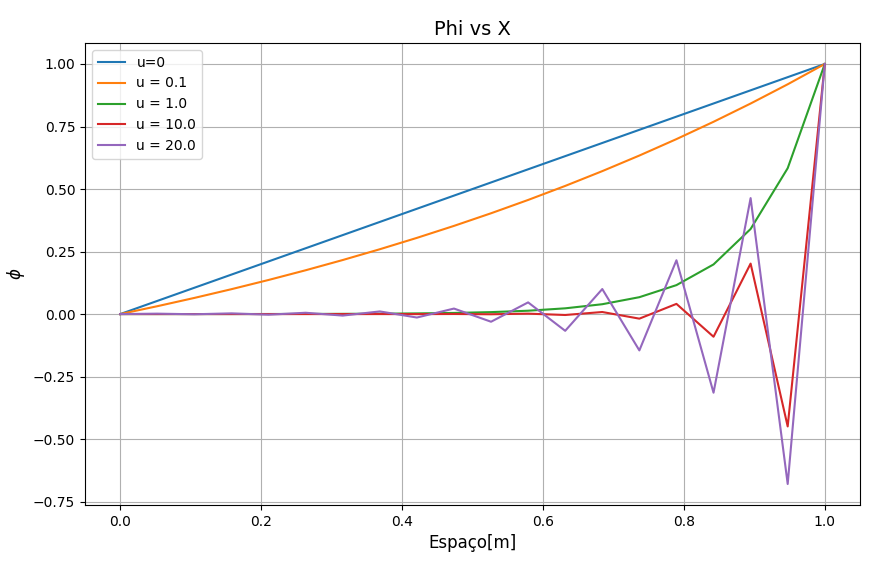
\includegraphics[width=.65\textwidth]{figures/43-1}
	\caption{Evolução do Phi no espaço CDS}
\end{figure}

Observam-se oscilações com velocidades maiores, devido à geração de coeficientes negativos por à utilização do CDS como sistema de interpolação espacial. O aumento da velocidade traz efeitos de difusão aumentados, que o CDS não trata adequadamente.\\

Incorporando UDS em termos advectivos

\begin{equation}
	\begin{aligned}
		\phi_e = \phi_p\\
		\phi_w = \phi_W\\
	\end{aligned}	
\end{equation}\\

\begin{figure}[H]
	\centering
	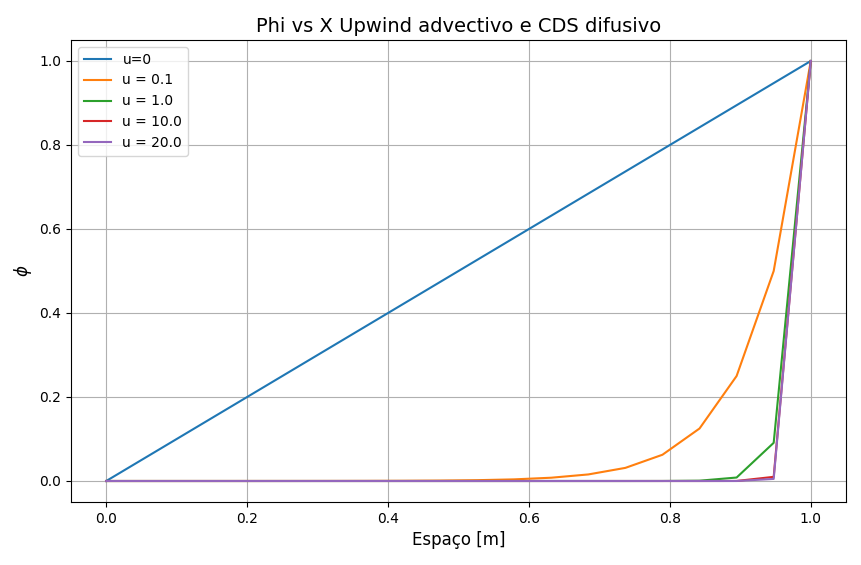
\includegraphics[width=.65\textwidth]{figures/43-2}
	\caption{Evolução do Phi no espaço UDS}
\end{figure}

A interpolação com o esquema Upwind elimina os efeitos dos coeficientes oscilatórios negativos do CDS. O gráfico mostra a evolução de phi, sempre positiva como esperado em um problema real advectivo difusivo.\\

Agora, utiliza-se o esquema exponencial dependente do número de peclet e compara-se com a equação exata da solução do problema dada pela equação 4.22 do livro do professor Maliska.

\begin{figure}[H]
	\centering
	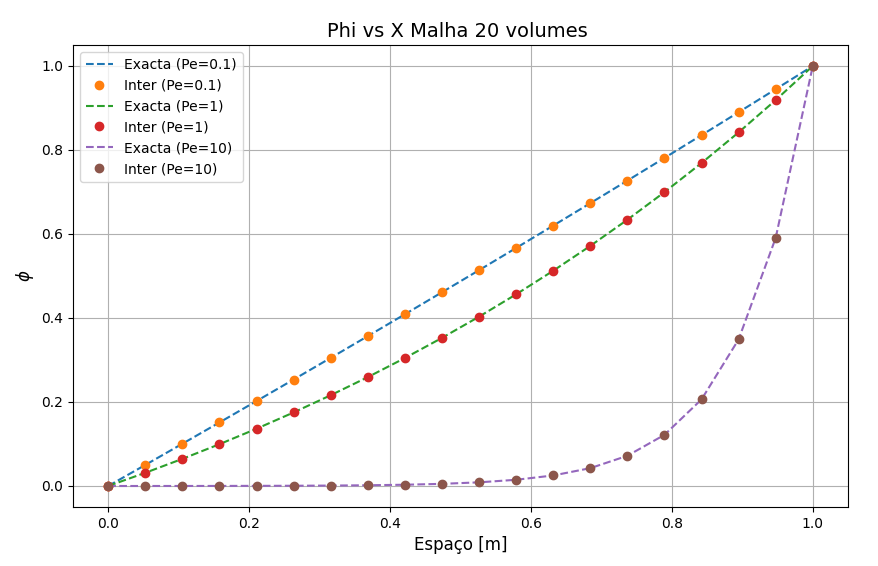
\includegraphics[width=.65\textwidth]{figures/43-3}
	\caption{Evolução do Phi com solução exata e exponencial para 20 volumes}
\end{figure}
\begin{figure}[H]
	\centering
	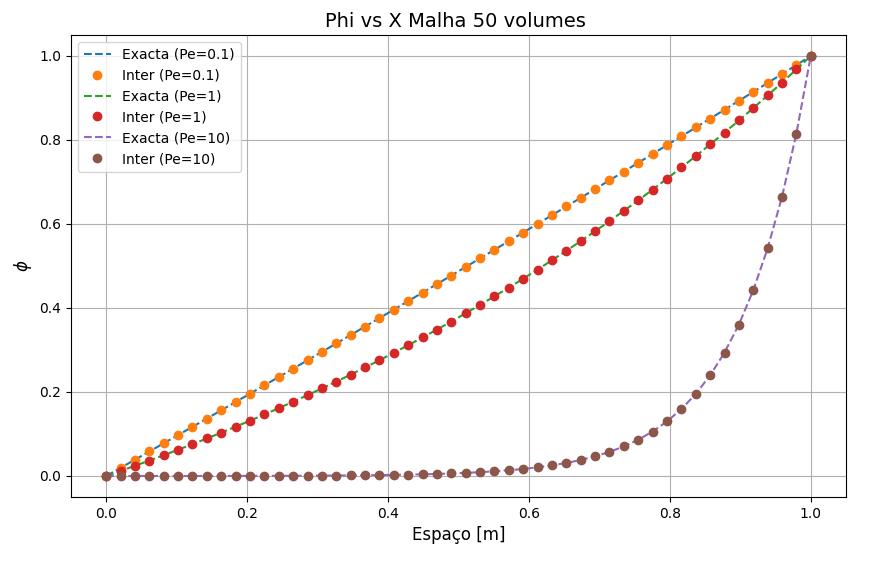
\includegraphics[width=.65\textwidth]{figures/43-4}
	\caption{Evolução do Phi com solução exata e exponencial para 50 volumes}
\end{figure}

Números de Peclet entre 0,1 e 10 são plotados para a solução exponencial e a solução exata. Dividindo o domínio com 20 e 50 volumes, nenhuma diferença é evidente nas soluções com malhas diferentes. Isso ocorre porque a função de interpolação do Esquema Exponencial é obtida precisamente a partir da mesma equação da solução exata sem gerar erros de truncamento.

Por fim, o caso é comparado com a utilização do esquema WUDS com os coeficientes dependentes do número de Peclet. Foram utilizadas duas malhas diferentes. Um gradiente melhor resolvido é evidente para os casos difusivos (baixo u) e uma ligeira diferença entre as duas malhas. A baixa dependência do refinamento da malha WUDS se deve à sua alta relação com o número de peclets, e a pequena diferença observada quando x é aproximadamente 1 pode estar associada a erros de truncamento entre as duas discrtizações espaciais.

\begin{figure}[H]
	\centering
	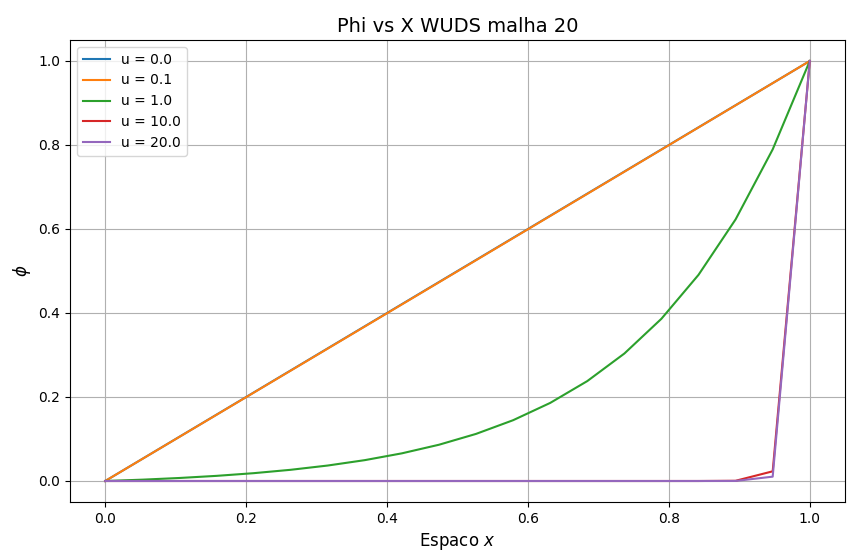
\includegraphics[width=.65\textwidth]{figures/43-5}
	\caption{Evolução do Phi com WUDS para 20 volumes}
\end{figure}

\begin{figure}[H]
	\centering
	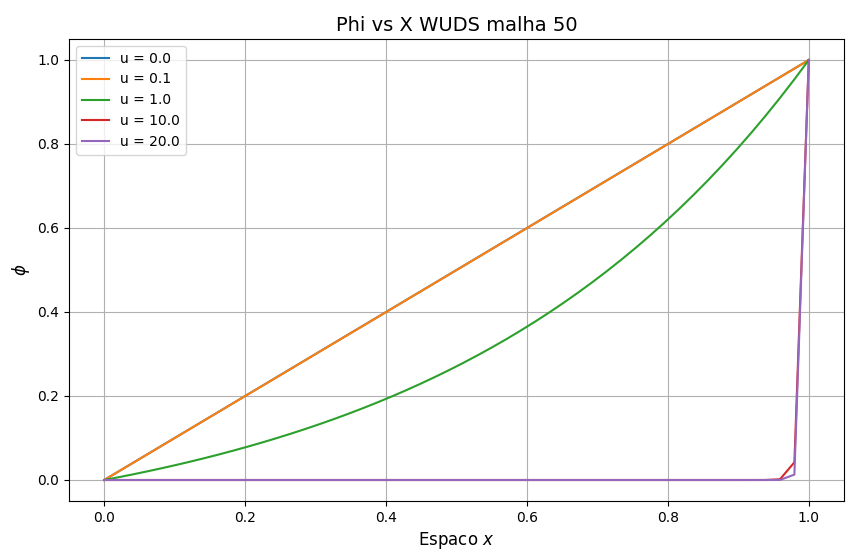
\includegraphics[width=.65\textwidth]{figures/43-6}
	\caption{Evolução do Phi com WUDS para 50 volumes}
\end{figure}

\section*{Exercício 3.2}
\subsubsection*{Para a equação de advecção-difusão 2D}

\begin{equation}
	\frac{\partial}{\partial t} (\rho \phi) + \frac{\partial}{\partial x} (\rho u \phi) + \frac{\partial}{\partial y} (\rho v \phi) = \frac{\partial}{\partial x} \left( \Gamma^\phi \frac{\partial \phi}{\partial x} \right) + \frac{\partial}{\partial y} \left( \Gamma^\phi \frac{\partial \phi}{\partial y} \right) + S^\phi
\end{equation}
Integrando-se no espaço e no tempo

\begin{equation}
	\begin{aligned}
		\frac{Mp \phi_{p} - Mp^{0}\phi_{p}^{0}}{\Delta t} + \rho u \phi\arrowvert_{e}\Delta y - \rho u \phi\arrowvert_{w}\Delta y + \rho v \phi\arrowvert_{n}\Delta x - \rho v \phi\arrowvert_{s}\Delta x = \\
		\varGamma^{\phi} \frac{\partial\phi}{\partial x}\bigg|^{\theta}_{e}\Delta y - \varGamma^{\phi} \frac{\partial\phi}{\partial x}\bigg|^{\theta}_{w}\Delta y + \varGamma^{\phi} \frac{\partial\phi}{\partial y}\bigg|^{\theta}_{n}\Delta y - \varGamma^{\phi} \frac{\partial\phi}{\partial y}\bigg|^{\theta}_{s}\Delta y + SpTp^{\theta} + Sc
	\end{aligned}
\end{equation}\\

\subsection*{CDS}

Aproximando os fluxos usando diferenças centrais CDS como interpolação linear, usamos as seguintes expressões

\begin{equation}
	\begin{aligned}
		\phi_{e} = \dfrac{\phi_{E} + \phi_{P}}{2} \\
		\phi_{w} = \dfrac{\phi_{W} + \phi_{P}}{2} \\
		\phi_{n} = \dfrac{\phi_{N} + \phi_{P}}{2} \\
		\phi_{s} = \dfrac{\phi_{S} + \phi_{P}}{2} \\
	\end{aligned}
\end{equation}

\begin{equation}
	\begin{aligned}
		\frac{\partial\phi}{\partial x}\bigg|_{e} = \frac{\phi_{E}-\phi_{P}}{\Delta x_{e}}\\
		\frac{\partial\phi}{\partial x}\bigg|_{w} = \frac{\phi_{P}-\phi_{W}}{\Delta x_{w}}\\
		\frac{\partial\phi}{\partial y}\bigg|_{n} = \frac{\phi_{N}-\phi_{P}}{\Delta x_{n}}\\
		\frac{\partial\phi}{\partial y}\bigg|_{s} = \frac{\phi_{P}-\phi_{S}}{\Delta x_{s}}
	\end{aligned}
\end{equation}
\\
Usando una formulacion implicita, o objetivo é converter a equação diferencial na equação linear da forma

\begin{equation}
	\begin{aligned}
		A_p\phi_p= A_e\phi_E + A_w\phi_W + A_n\phi_N - A_s\phi_S + A_p^{0}\phi_P^{0} + B_P
	\end{aligned}
\end{equation}\\

Os coeficientes que acompanham phi em cada face são calculados, ficando>

\begin{equation}
	\begin{aligned}
		Ap = \frac{M_P}{\Delta t} + A_e + A_w + A_s + A_n - S_P\Delta x \Delta y\\
		A_e = \varGamma^{\theta}\frac{\Delta y}{\Delta x} + \frac{\rho u \Delta y}{2}\\
		A_w = \varGamma^{\theta}\frac{\Delta y}{\Delta x} - \frac{\rho u \Delta y}{2}\\
		A_n = \varGamma^{\theta}\frac{\Delta x}{\Delta y} + \frac{\rho v \Delta x}{2}\\
		A_s = \varGamma^{\theta}\frac{\Delta x}{\Delta y} + \frac{\rho v \Delta x}{2}\\
		B_p = Sc\Delta x \Delta y \Delta t + \frac{M_P^{0}\phi_p^{0}}{\Delta t}\Delta x \Delta y
	\end{aligned}
\end{equation}\\

Usando valores unitários de densidade (cte), difusividade (cte) e espaçamento em x e y, os valores de velocidade são variados para calcular os valores da matriz do sistema que resolve o problema difusivo advectivo. As matrizes para uma malha 5 x 5 os casos de $ Pe = 10 $ e $ Pe = 1000$ estão relacionadas.\\

Para $ Pe = 10 $ ($u = 10$)

\begin{table}[H]
	\centering
	\begin{tabular}{|c|c|c|c|c|c|c|}
		\hline
		\textbf{Vol} & \textbf{Ap} & \textbf{Ae} & \textbf{Aw} & \textbf{An} & \textbf{As} & \textbf{Bp} \\
		\hline
		1,1  & 15.5 & 6.0  & 0.0  & 0.0  & 0.5  & 11.0 \\
		1,2  & 11.5 & 6.0  & \textcolor{red}{-4.0} & 0.0  & 0.5  & 11.0 \\
		1,3  & 11.5 & 6.0  & \textcolor{red}{-4.0} & 0.0  & 0.5  & 11.0 \\
		1,4  & 11.5 & 6.0  & \textcolor{red}{-4.0} & 0.0  & 0.5  & 11.0 \\
		1,5  & 5.5  & 0.0  & \textcolor{red}{-4.0} & 0.0  & 0.5  & 11.0 \\
		2,1  & 17.0 & 6.0  & 0.0  & 1.5  & 0.5  & 11.0 \\
		2,2  & 13.0 & 6.0  & \textcolor{red}{-4.0} & 1.5  & 0.5  & 11.0 \\
		2,3  & 13.0 & 6.0  & \textcolor{red}{-4.0} & 1.5  & 0.5  & 11.0 \\
		2,4  & 13.0 & 6.0  & \textcolor{red}{-4.0} & 1.5  & 0.5  & 11.0 \\
		2,5  & 7.0  & 0.0  & \textcolor{red}{-4.0} & 1.5  & 0.5  & 11.0 \\
		3,1  & 17.0 & 6.0  & 0.0  & 1.5  & 0.5  & 11.0 \\
		3,2  & 13.0 & 6.0  & \textcolor{red}{-4.0} & 1.5  & 0.5  & 11.0 \\
		3,3  & 13.0 & 6.0  & \textcolor{red}{-4.0} & 1.5  & 0.5  & 11.0 \\
		3,4  & 13.0 & 6.0  & \textcolor{red}{-4.0} & 1.5  & 0.5  & 11.0 \\
		3,5  & 7.0  & 0.0  & \textcolor{red}{-4.0} & 1.5  & 0.5  & 11.0 \\
		4,1  & 17.0 & 6.0  & 0.0  & 1.5  & 0.5  & 11.0 \\
		4,2  & 13.0 & 6.0  & \textcolor{red}{-4.0} & 1.5  & 0.5  & 11.0 \\
		4,3  & 13.0 & 6.0  & \textcolor{red}{-4.0} & 1.5  & 0.5  & 11.0 \\
		4,4  & 13.0 & 6.0  & \textcolor{red}{-4.0} & 1.5  & 0.5  & 11.0 \\
		4,5  & 7.0  & 0.0  & \textcolor{red}{-4.0} & 1.5  & 0.5  & 11.0 \\
		5,1  & 16.5 & 6.0  & 0.0  & 1.5  & 0.0  & 11.0 \\
		5,2  & 12.5 & 6.0  & \textcolor{red}{-4.0} & 1.5  & 0.0  & 11.0 \\
		5,3  & 12.5 & 6.0  & \textcolor{red}{-4.0} & 1.5  & 0.0  & 11.0 \\
		5,4  & 12.5 & 6.0  & \textcolor{red}{-4.0} & 1.5  & 0.0  & 11.0 \\
		5,5  & 6.5  & 0.0  & \textcolor{red}{-4.0} & 1.5  & 0.0  & 11.0 \\
		\hline
	\end{tabular}
	\caption{Coeficientes calculados para sistema CDS com Pe=10}
\end{table}

Observam-se valores relativamente estáveis e simétricos dada a participação tanto dos efeitos difusivos quanto dos advectivos. Os valores dos coeficientes para as faces Aw e Ae são de maior magnitude devido à advecção no fluxo a montante e a jusante de P\\

Para $ Pe = 1000 $ ($u = 1000$)
\begin{table}[H]
	\centering
	\begin{tabular}{|c|c|c|c|c|c|c|}
		\hline
		\textbf{Vol} & \textbf{Ap} & \textbf{Ae} & \textbf{Aw} & \textbf{An} & \textbf{As} & \textbf{Bp} \\
		\hline
		1,1 & 510.5  & 501.0  & 0.0  & 0.0  & 0.5  & 11.0 \\
		1,2 & 11.5   & 501.0  & \textcolor{red}{-499.0} & 0.0  & 0.5  & 11.0 \\
		1,3 & 11.5   & 501.0  & \textcolor{red}{-499.0} & 0.0  & 0.5  & 11.0 \\
		1,4 & 11.5   & 501.0  & \textcolor{red}{-499.0} & 0.0  & 0.5  & 11.0 \\
		1,5 & \textcolor{red}{-489.5}  & 0.0  & \textcolor{red}{-499.0} & 0.0  & 0.5  & 11.0 \\
		2,1 & 512.0  & 501.0  & 0.0  & 1.5  & 0.5  & 11.0 \\
		2,2 & 13.0   & 501.0  & \textcolor{red}{-499.0} & 1.5  & 0.5  & 11.0 \\
		2,3 & 13.0   & 501.0  & \textcolor{red}{-499.0} & 1.5  & 0.5  & 11.0 \\
		2,4 & 13.0   & 501.0  & \textcolor{red}{-499.0} & 1.5  & 0.5  & 11.0 \\
		2,5 & \textcolor{red}{-488.0}  & 0.0  & \textcolor{red}{-499.0} & 1.5  & 0.5  & 11.0 \\
		3,1 & 512.0  & 501.0  & 0.0  & 1.5  & 0.5  & 11.0 \\
		3,2 & 13.0   & 501.0  & \textcolor{red}{-499.0} & 1.5  & 0.5  & 11.0 \\
		3,3 & 13.0   & 501.0  & \textcolor{red}{-499.0} & 1.5  & 0.5  & 11.0 \\
		3,4 & 13.0   & 501.0  & \textcolor{red}{-499.0} & 1.5  & 0.5  & 11.0 \\
		3,5 & \textcolor{red}{-488.0}  & 0.0  & \textcolor{red}{-499.0} & 1.5  & 0.5  & 11.0 \\
		4,1 & 512.0  & 501.0  & 0.0  & 1.5  & 0.5  & 11.0 \\
		4,2 & 13.0   & 501.0  & \textcolor{red}{-499.0} & 1.5  & 0.5  & 11.0 \\
		4,3 & 13.0   & 501.0  & \textcolor{red}{-499.0} & 1.5  & 0.5  & 11.0 \\
		4,4 & 13.0   & 501.0  & \textcolor{red}{-499.0} & 1.5  & 0.5  & 11.0 \\
		4,5 & \textcolor{red}{-488.0}  & 0.0  & \textcolor{red}{-499.0} & 1.5  & 0.5  & 11.0 \\
		5,1 & 511.5  & 501.0  & 0.0  & 1.5  & 0.0  & 11.0 \\
		5,2 & 12.5   & 501.0  & \textcolor{red}{-499.0} & 1.5  & 0.0  & 11.0 \\
		5,3 & 12.5   & 501.0  & \textcolor{red}{-499.0} & 1.5  & 0.0  & 11.0 \\
		5,4 & 12.5   & 501.0  & \textcolor{red}{-499.0} & 1.5  & 0.0  & 11.0 \\
		5,5 & \textcolor{red}{-488.5}  & 0.0  & \textcolor{red}{-499.0} & 1.5  & 0.0  & 11.0 \\
		\hline
	\end{tabular}
	\caption{Coeficientes calculados para sistema CDS com Pe=1000}
\end{table}

	
Com o aumento da velocidade horizontal (Número de Peclet) o problema é fortemente dominado pela advecção em x. Valores elevados de Ae e Aw modificam consideravelmente o valor de Ap, causando valores negativos que também trazem instabilidade numérica. O sistema CDS é mais consistente para casos de dominância difusiva.
	
\subsection*{UDS}

Para o esquema UPWIND, as funções de interpolação têm as seguintes expressões para $u > 0$ e $ v > 0$

\begin{equation}
	\begin{aligned}
		\phi_e = \phi_p\\
		\phi_w = \phi_W\\
		\phi_n = \phi_p\\
		\phi_s = \phi_S
	\end{aligned}	
\end{equation}\\

\begin{equation}
	\begin{aligned}
		A_e = \varGamma^{\theta}\frac{\Delta y}{\Delta x} \\
		A_w = \varGamma^{\theta}\frac{\Delta y}{\Delta x} - \frac{\rho u \Delta y}{2}\\
		A_n = \varGamma^{\theta}\frac{\Delta x}{\Delta y}\\
		A_s = \varGamma^{\theta}\frac{\Delta x}{\Delta y} + \frac{\rho v \Delta x}{2}
	\end{aligned}
\end{equation}\\

Deixando a solução do efeito advectivo no termo a jusante da discretização. Agora as matrizes assumem os seguintes valores

\begin{table}[H]
	\centering
	\begin{tabular}{|c|c|c|c|c|c|c|}
		\hline
		\textbf{Vol} & \textbf{Ap} & \textbf{Ae} & \textbf{Aw} & \textbf{An} & \textbf{As} & \textbf{Bp} \\
		\hline
		1,1  & 24.0  & 1.0  & 11.0  & 1.0  & 2.0  & 11.0 \\
		1,2  & 24.0  & 1.0  & 11.0  & 1.0  & 2.0  & 11.0 \\
		1,3  & 24.0  & 1.0  & 11.0  & 1.0  & 2.0  & 11.0 \\
		1,4  & 24.0  & 1.0  & 11.0  & 1.0  & 2.0  & 11.0 \\
		1,5  & 24.0  & 1.0  & 11.0  & 1.0  & 2.0  & 11.0 \\
		2,1  & 24.0  & 1.0  & 11.0  & 1.0  & 2.0  & 11.0 \\
		2,2  & 24.0  & 1.0  & 11.0  & 1.0  & 2.0  & 11.0 \\
		2,3  & 24.0  & 1.0  & 11.0  & 1.0  & 2.0  & 11.0 \\
		2,4  & 24.0  & 1.0  & 11.0  & 1.0  & 2.0  & 11.0 \\
		2,5  & 24.0  & 1.0  & 11.0  & 1.0  & 2.0  & 11.0 \\
		3,1  & 24.0  & 1.0  & 11.0  & 1.0  & 2.0  & 11.0 \\
		3,2  & 24.0  & 1.0  & 11.0  & 1.0  & 2.0  & 11.0 \\
		3,3  & 24.0  & 1.0  & 11.0  & 1.0  & 2.0  & 11.0 \\
		3,4  & 24.0  & 1.0  & 11.0  & 1.0  & 2.0  & 11.0 \\
		3,5  & 24.0  & 1.0  & 11.0  & 1.0  & 2.0  & 11.0 \\
		4,1  & 24.0  & 1.0  & 11.0  & 1.0  & 2.0  & 11.0 \\
		4,2  & 24.0  & 1.0  & 11.0  & 1.0  & 2.0  & 11.0 \\
		4,3  & 24.0  & 1.0  & 11.0  & 1.0  & 2.0  & 11.0 \\
		4,4  & 24.0  & 1.0  & 11.0  & 1.0  & 2.0  & 11.0 \\
		4,5  & 24.0  & 1.0  & 11.0  & 1.0  & 2.0  & 11.0 \\
		5,1  & 22.0  & 1.0  & 11.0  & 1.0  & 0.0  & 11.0 \\
		5,2  & 22.0  & 1.0  & 11.0  & 1.0  & 0.0  & 11.0 \\
		5,3  & 22.0  & 1.0  & 11.0  & 1.0  & 0.0  & 11.0 \\
		5,4  & 22.0  & 1.0  & 11.0  & 1.0  & 0.0  & 11.0 \\
		5,5  & 22.0  & 1.0  & 11.0  & 1.0  & 0.0  & 11.0 \\
		\hline
	\end{tabular}
	\caption{Coeficientes calculados para sistema UDS com Pe=10}
\end{table}

\begin{table}[H]
	\centering
	\begin{tabular}{|c|c|c|c|c|c|c|}
		\hline
		\textbf{Vol} & \textbf{Ap} & \textbf{Ae} & \textbf{Aw} & \textbf{An} & \textbf{As} & \textbf{Bp} \\
		\hline
		1,1  & 1014.0  & 1.0  & 1001.0  & 1.0  & 2.0  & 11.0 \\
		1,2  & 1014.0  & 1.0  & 1001.0  & 1.0  & 2.0  & 11.0 \\
		1,3  & 1014.0  & 1.0  & 1001.0  & 1.0  & 2.0  & 11.0 \\
		1,4  & 1014.0  & 1.0  & 1001.0  & 1.0  & 2.0  & 11.0 \\
		1,5  & 1014.0  & 1.0  & 1001.0  & 1.0  & 2.0  & 11.0 \\
		2,1  & 1014.0  & 1.0  & 1001.0  & 1.0  & 2.0  & 11.0 \\
		2,2  & 1014.0  & 1.0  & 1001.0  & 1.0  & 2.0  & 11.0 \\
		2,3  & 1014.0  & 1.0  & 1001.0  & 1.0  & 2.0  & 11.0 \\
		2,4  & 1014.0  & 1.0  & 1001.0  & 1.0  & 2.0  & 11.0 \\
		2,5  & 1014.0  & 1.0  & 1001.0  & 1.0  & 2.0  & 11.0 \\
		3,1  & 1014.0  & 1.0  & 1001.0  & 1.0  & 2.0  & 11.0 \\
		3,2  & 1014.0  & 1.0  & 1001.0  & 1.0  & 2.0  & 11.0 \\
		3,3  & 1014.0  & 1.0  & 1001.0  & 1.0  & 2.0  & 11.0 \\
		3,4  & 1014.0  & 1.0  & 1001.0  & 1.0  & 2.0  & 11.0 \\
		3,5  & 1014.0  & 1.0  & 1001.0  & 1.0  & 2.0  & 11.0 \\
		4,1  & 1014.0  & 1.0  & 1001.0  & 1.0  & 2.0  & 11.0 \\
		4,2  & 1014.0  & 1.0  & 1001.0  & 1.0  & 2.0  & 11.0 \\
		4,3  & 1014.0  & 1.0  & 1001.0  & 1.0  & 2.0  & 11.0 \\
		4,4  & 1014.0  & 1.0  & 1001.0  & 1.0  & 2.0  & 11.0 \\
		4,5  & 1014.0  & 1.0  & 1001.0  & 1.0  & 2.0  & 11.0 \\
		5,1  & 1012.0  & 1.0  & 1001.0  & 1.0  & 0.0  & 11.0 \\
		5,2  & 1012.0  & 1.0  & 1001.0  & 1.0  & 0.0  & 11.0 \\
		5,3  & 1012.0  & 1.0  & 1001.0  & 1.0  & 0.0  & 11.0 \\
		5,4  & 1012.0  & 1.0  & 1001.0  & 1.0  & 0.0  & 11.0 \\
		5,5  & 1012.0  & 1.0  & 1001.0  & 1.0  & 0.0  & 11.0 \\
		\hline
	\end{tabular}
	\caption{Coeficientes calculados para sistema UDS com Pe=1000}
\end{table}

A implementação da interpolação Upstream mitiga a geração de valores negativos. Portanto, a estabilidade numérica é boa e não há oscilações em problemas advectivos fortes. Porém, como observado no caso de maior advecção, a interpolação é orientada para os termos a jusante (Aw), fazendo com que não capture adequadamente gradientes elevados.

\subsection*{QUICK}

Para o caso de Upwind Quadratica, são utilizadas expressões que aumentam a ordem de aproximação do CDS com as seguintes expressões para $u > 0$

\begin{equation}
	\begin{aligned}
		\phi_e = -\dfrac{1}{8}\phi_W +\dfrac{1}{6}\phi_P +\dfrac{1}{8}\phi_E \\
		\phi_n = -\dfrac{1}{8}\phi_S +\dfrac{1}{6}\phi_P +\dfrac{1}{8}\phi_N
	\end{aligned}
\end{equation}\\

Os valores das matrices fican

\begin{table}[H]
	\centering
	\begin{tabular}{|c|c|c|c|c|c|c|}
		\hline
		\textbf{Vol} & \textbf{Ap} & \textbf{Ae} & \textbf{Aw} & \textbf{An} & \textbf{As} & \textbf{Bp} \\
		\hline
		1,1  & 14.75  & 4.75  & 0.00  & 1.0  & 0.0  & 11.0 \\
		1,2  & 13.50  & 4.75  & -1.25 & 1.0  & 0.0  & 11.0 \\
		1,3  & 13.50  & 4.75  & -1.25 & 1.0  & 0.0  & 11.0 \\
		1,4  & 13.50  & 4.75  & -1.25 & 1.0  & 0.0  & 11.0 \\
		1,5  & 9.75   & 1.00  & -1.25 & 1.0  & 0.0  & 11.0 \\
		2,1  & 15.75  & 4.75  & 0.00  & 2.0  & 0.0  & 11.0 \\
		2,2  & 14.50  & 4.75  & -1.25 & 2.0  & 0.0  & 11.0 \\
		2,3  & 14.50  & 4.75  & -1.25 & 2.0  & 0.0  & 11.0 \\
		2,4  & 14.50  & 4.75  & -1.25 & 2.0  & 0.0  & 11.0 \\
		2,5  & 10.75  & 1.00  & -1.25 & 2.0  & 0.0  & 11.0 \\
		3,1  & 15.75  & 4.75  & 0.00  & 2.0  & 0.0  & 11.0 \\
		3,2  & 14.50  & 4.75  & -1.25 & 2.0  & 0.0  & 11.0 \\
		3,3  & 14.50  & 4.75  & -1.25 & 2.0  & 0.0  & 11.0 \\
		3,4  & 14.50  & 4.75  & -1.25 & 2.0  & 0.0  & 11.0 \\
		3,5  & 10.75  & 1.00  & -1.25 & 2.0  & 0.0  & 11.0 \\
		4,1  & 15.75  & 4.75  & 0.00  & 2.0  & 0.0  & 11.0 \\
		4,2  & 14.50  & 4.75  & -1.25 & 2.0  & 0.0  & 11.0 \\
		4,3  & 14.50  & 4.75  & -1.25 & 2.0  & 0.0  & 11.0 \\
		4,4  & 14.50  & 4.75  & -1.25 & 2.0  & 0.0  & 11.0 \\
		4,5  & 10.75  & 1.00  & -1.25 & 2.0  & 0.0  & 11.0 \\
		5,1  & 16.75  & 4.75  & 0.00  & 2.0  & 1.0  & 11.0 \\
		5,2  & 15.50  & 4.75  & -1.25 & 2.0  & 1.0  & 11.0 \\
		5,3  & 15.50  & 4.75  & -1.25 & 2.0  & 1.0  & 11.0 \\
		5,4  & 15.50  & 4.75  & -1.25 & 2.0  & 1.0  & 11.0 \\
		5,5  & 11.75  & 1.00  & -1.25 & 2.0  & 1.0  & 11.0 \\
		\hline
	\end{tabular}
	\caption{Coeficientes calculados para sistema QUICK com Pe=10}
\end{table}


\begin{table}[H]
	\centering
	\begin{tabular}{|c|c|c|c|c|c|c|}
		\hline
		\textbf{Vol} & \textbf{Ap} & \textbf{Ae} & \textbf{Aw} & \textbf{An} & \textbf{As} & \textbf{Bp} \\
		\hline
		1,1  & 386.0  & 376.0  & 0.0  & 1.0  & 0.0  & 11.0 \\
		1,2  & 261.0  & 376.0  & -125.0 & 1.0  & 0.0  & 11.0 \\
		1,3  & 261.0  & 376.0  & -125.0 & 1.0  & 0.0  & 11.0 \\
		1,4  & 261.0  & 376.0  & -125.0 & 1.0  & 0.0  & 11.0 \\
		1,5  & -114.0 & 1.0    & -125.0 & 1.0  & 0.0  & 11.0 \\
		2,1  & 387.0  & 376.0  & 0.0  & 2.0  & 0.0  & 11.0 \\
		2,2  & 262.0  & 376.0  & -125.0 & 2.0  & 0.0  & 11.0 \\
		2,3  & 262.0  & 376.0  & -125.0 & 2.0  & 0.0  & 11.0 \\
		2,4  & 262.0  & 376.0  & -125.0 & 2.0  & 0.0  & 11.0 \\
		2,5  & -113.0 & 1.0    & -125.0 & 2.0  & 0.0  & 11.0 \\
		3,1  & 387.0  & 376.0  & 0.0  & 2.0  & 0.0  & 11.0 \\
		3,2  & 262.0  & 376.0  & -125.0 & 2.0  & 0.0  & 11.0 \\
		3,3  & 262.0  & 376.0  & -125.0 & 2.0  & 0.0  & 11.0 \\
		3,4  & 262.0  & 376.0  & -125.0 & 2.0  & 0.0  & 11.0 \\
		3,5  & -113.0 & 1.0    & -125.0 & 2.0  & 0.0  & 11.0 \\
		4,1  & 387.0  & 376.0  & 0.0  & 2.0  & 0.0  & 11.0 \\
		4,2  & 262.0  & 376.0  & -125.0 & 2.0  & 0.0  & 11.0 \\
		4,3  & 262.0  & 376.0  & -125.0 & 2.0  & 0.0  & 11.0 \\
		4,4  & 262.0  & 376.0  & -125.0 & 2.0  & 0.0  & 11.0 \\
		4,5  & -113.0 & 1.0    & -125.0 & 2.0  & 0.0  & 11.0 \\
		5,1  & 388.0  & 376.0  & 0.0  & 2.0  & 1.0  & 11.0 \\
		5,2  & 263.0  & 376.0  & -125.0 & 2.0  & 1.0  & 11.0 \\
		5,3  & 263.0  & 376.0  & -125.0 & 2.0  & 1.0  & 11.0 \\
		5,4  & 263.0  & 376.0  & -125.0 & 2.0  & 1.0  & 11.0 \\
		5,5  & -112.0 & 1.0    & -125.0 & 2.0  & 1.0  & 11.0 \\
		\hline
	\end{tabular}
	\caption{Coeficientes calculados para sistema QUICK com Pe=1000}
\end{table}

O QUICK, como ter um sistema de interpolação ponderada com os coeficientes que acompanham cada termo, lida melhor com valores negativos (menores) que o sistema CDS. No entanto, ambos os sistemas produzem distribuições matriciais semelhantes, onde o caso advectivo forte mostra mais oscilação do que o caso advectivo difusivo.

\section*{Exercício 3.3}
O problema de advecção pura bidimensional em regimen permanente começa na equação


\begin{equation}
	\begin{aligned}
		\frac{\partial}{\partial x} (\rho u \phi) + \frac{\partial}{\partial y} (\rho v \phi) = 0
	\end{aligned}
\end{equation}\\


\begin{figure}[H]
	\centering
	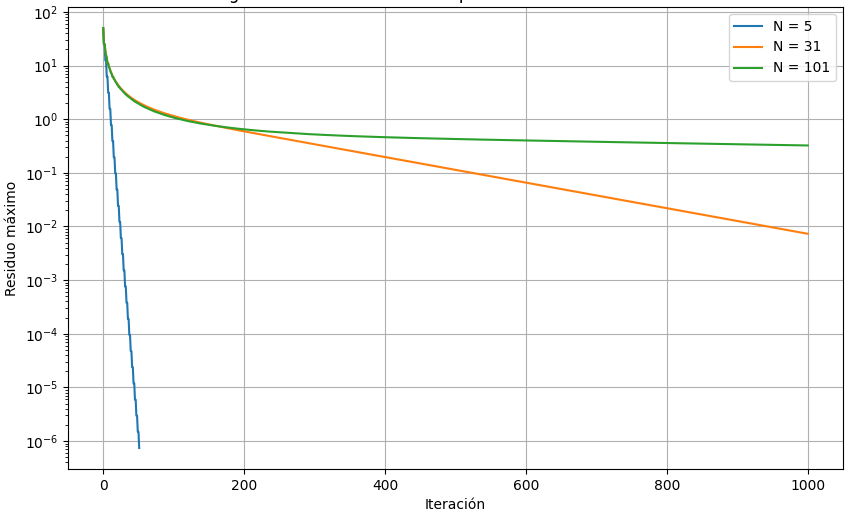
\includegraphics[width=.65\textwidth]{figures/3-1}
	\caption{Problema advectivo com condicoes de contorno}
\end{figure}
Integrando-se no espaço e no tempo

\subsection*{CDS}

\begin{equation}
	\begin{aligned}
		\rho u \phi\arrowvert_{e}\Delta y - \rho u \phi\arrowvert_{w}\Delta y + \rho v \phi\arrowvert_{n}\Delta x - \rho v \phi\arrowvert_{s}\Delta x 
	\end{aligned}
\end{equation}\\

Aproximando os fluxos usando diferenças centrais CDS como interpolação linear, usamos as seguintes expressões para cada colume de control

\begin{equation}
	\begin{aligned}
		\phi_{e} = \dfrac{\phi_{E} + \phi_{P}}{2} \\
		\phi_{w} = \dfrac{\phi_{W} + \phi_{P}}{2} \\
		\phi_{n} = \dfrac{\phi_{N} + \phi_{P}}{2} \\
		\phi_{s} = \dfrac{\phi_{S} + \phi_{P}}{2} \\
	\end{aligned}
\end{equation}

O objetivo é converter a equação diferencial na equação linear da forma

\begin{equation}
	\begin{aligned}
		A_p\phi_p= A_e\phi_E + A_w\phi_W + A_n\phi_N + A_s\phi_S 
	\end{aligned}
\end{equation}\\

Os coeficientes que acompanham phi em cada face são calculados, ficando

\begin{equation}
	\begin{aligned}
		Ap = A_e + A_w + A_s + A_n\\
		A_e = \frac{\rho u \Delta y}{2}\\
		A_w = \frac{\rho u \Delta y}{2}\\
		A_n = \frac{\rho v \Delta x}{2}\\
		A_s = \frac{\rho v \Delta x}{2}\\
	\end{aligned}
\end{equation}\\

Usando valores unitários de densidade (cte), espaçamento em x e y, em velocidades. É apresentado como os diferentes esquemas de interpolação resolvem este problema advectivo com as condições de contorno descritas na Figura 1.

\begin{figure}[H]
	\centering
	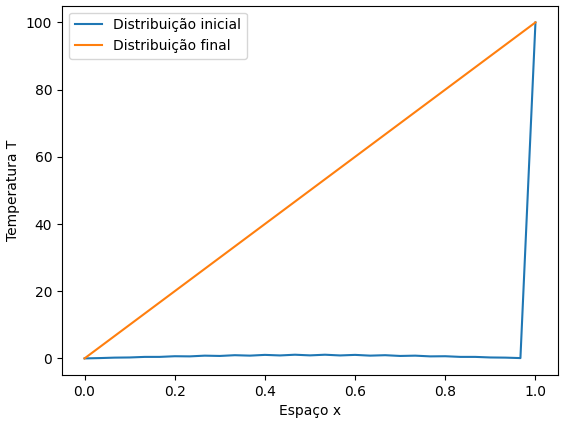
\includegraphics[width=.65\textwidth]{figures/3-3}
	\caption{Contorno de $\phi$ com malha 50 x 50 volumes esquema CDS}
\end{figure}

\begin{figure}[H]
	\centering
	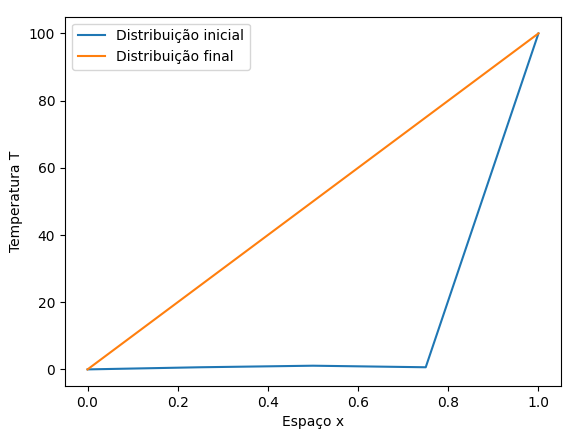
\includegraphics[width=.65\textwidth]{figures/3-2}
	\caption{Oscilaciones de $\phi$ em diagonal com esquema CDS}
\end{figure}


Como visto no problema advectivo difusivo, o sistema CDS não funciona bem com problemas de dominância advectiva, onde os erros de truncamento nao dissipativos produzir oscilações numéricas. Como exemplo, é apresentado o caso da malha de volume 50 x 50 (utilizando transiente distorcido) onde são observadas fortes oscilações da variável transportada ao longo da diagonal de interesse.

\subsection*{UDS}

Sustituindo os valores Upstreamen na equaçao discretizada


\begin{equation}
	\begin{aligned}
		\phi_e = \phi_P\\
		\phi_w = \phi_W\\
		\phi_n = \phi_P\\
		\phi_s = \phi_S
	\end{aligned}	
\end{equation}\\

Obtem-se os contornos e a evolução de phi para os casos\\

\begin{figure}[H]
	\centering
	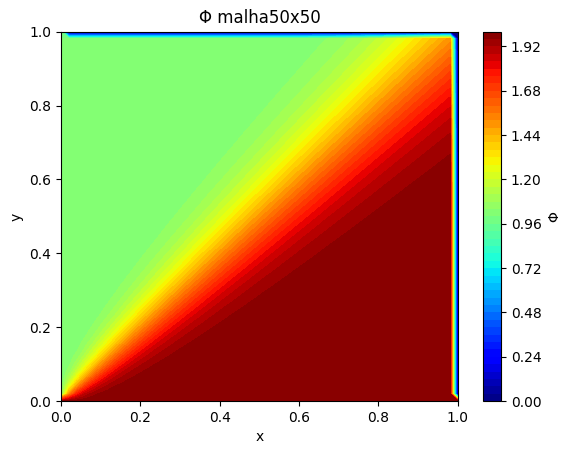
\includegraphics[width=.65\textwidth]{figures/3-4}
	\caption{Contorno de phi com malha de 50 x 50 volumes}
\end{figure}

\begin{figure}[H]
	\centering
	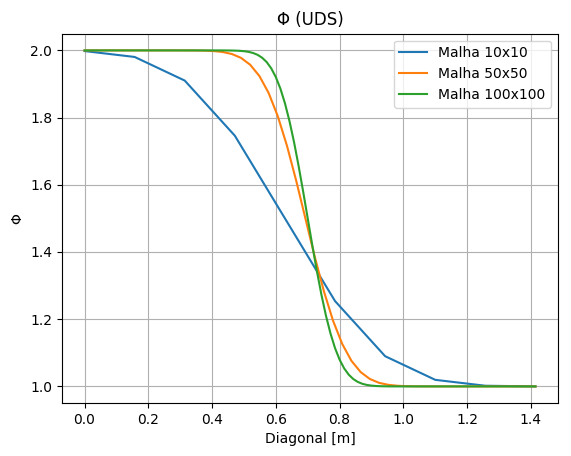
\includegraphics[width=.65\textwidth]{figures/3-5}
	\caption{Evolução de $\phi$ em diagonal com esquema CDS}
\end{figure}

O sistema de interpolação UDS resolve o problema de oscilação numérica, trazendo o efeito de suavização de gradientes devido ao aparecimento de erros de truncamento dissipativos que resultam em difusão numérica. Pode-se observar como a difusão diminui com refinamento especial (reduzindo imprecisões). Porém, com um refinamento bem discreto (100 x 100) o gradiente ainda é visível, pois utilizamos interpolação com erros de truncamento dissipativos em um problema advectivo.

\subsection*{WUDS}

E incorporado o sistema WUDS dependente do número de Peclet, acrescentando o termo alfa ao termo convectivo. Uma análise da diferença com a velocidade foi feita aumentando v=2, verificando os resultados do WUDS com um número de peclets maior. Foi encontrada uma pequena diferença, esperando-se uma melhor captação do gradiente.

\begin{figure}[H]
	\centering
	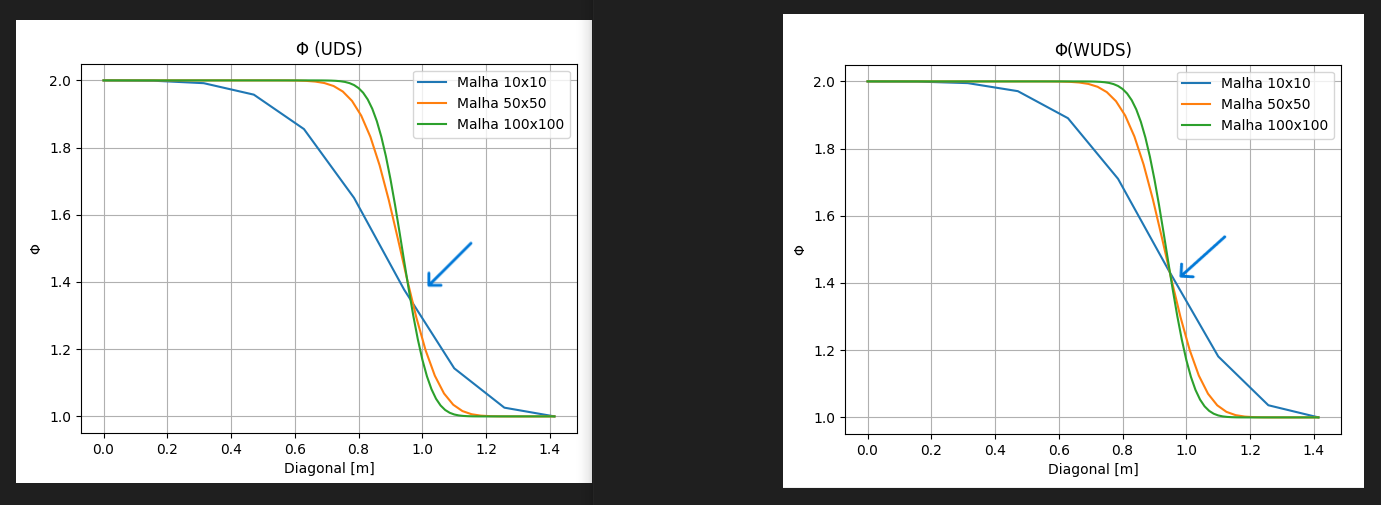
\includegraphics[width=.65\textwidth]{figures/3-7}
	\caption{Evolução de $\phi$ em diagonal com esquema WUDS}
\end{figure}

\end{document}





